\section{Seller guide} \label{_venditore}
\subsection{Purpose of the section}
The goal of this section of the document is to describe what a seller can do using EmporioLambda.

\subsection{How access to the seller dashboard} \label{_dashboard}

\subsection{How to add a product}
In order to add a product, from the \hyperref[_dashboard]{dashboard} click the Manage your products button.
\begin{figure}[H]
    \centering
    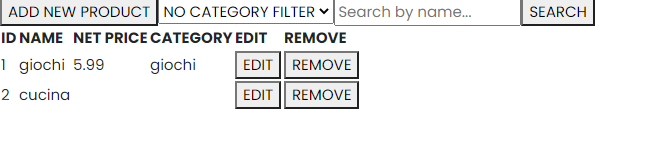
\includegraphics[width=\linewidth]{res/images/venditore/manageproducts.png}
    \caption{Manage products}
\end{figure}

\subsection{How to edit a product}
In order to add a product, from the \hyperref[_dashboard]{dashboard} click the Manage your products button.
\begin{figure}[H]
    \centering
    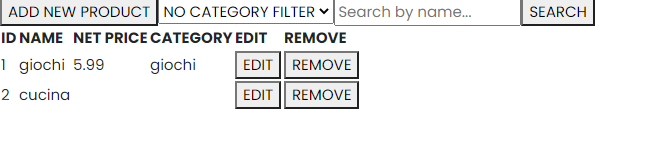
\includegraphics[width=\linewidth]{res/images/venditore/manageproducts.png}
    \caption{Edit prouct products}
\end{figure}

\subsection{How to remove a product}
In order to add a product, from the \hyperref[_dashboard]{dashboard} click the Manage your products button.
\begin{figure}[H]
    \centering
    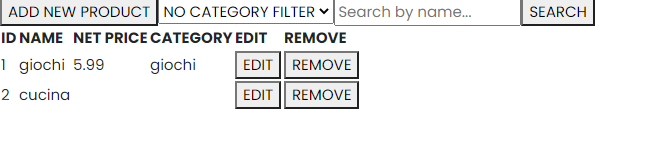
\includegraphics[width=\linewidth]{res/images/venditore/manageproducts.png}
    \caption{Manage products}
\end{figure}

